\todo{CS4002}
\todo[color=blue!40]{CS4003}
\todo[color=green!40]{CS4004}

En este capítulo se introducen los conceptos necesarios para la revisión de la literatura y el desarrollo de la propuesta de investigación. Para ello, se explican definiciones y conceptos importantes como descriptores, correspondencia, alineación y redes neuronales aplicadas a modelos 3D.

\section{Descriptores}

\subsection{Descriptor \textit{surflet-pair-relation} extendido (ESPR)}
El descriptor ESPR de un par de puntos orientados $(\mathbf{u},\mathbf{v})$ está definido por $\mathbf{S}_{uv} = \{\alpha, \beta, \theta, d, d_g\}$. Los parámetros $\alpha$ y $\beta$ son los ángulos entre las normales $n_u$, $n_v$ y la línea $p_up_v$. El ángulo $\theta$ está formado entre la proyección de las normales en un plano $\Gamma$ perpendicular a $p_up_v$. Las distancias $d$ y $d_g$ representan la distancia euclidiana y geodésica entre $p_u$ y $p_v$ \cite{fn2}. Los parámetros se ilustran en la figura \ref{fig:espr}.

\begin{figure}[!h]
    \centering
    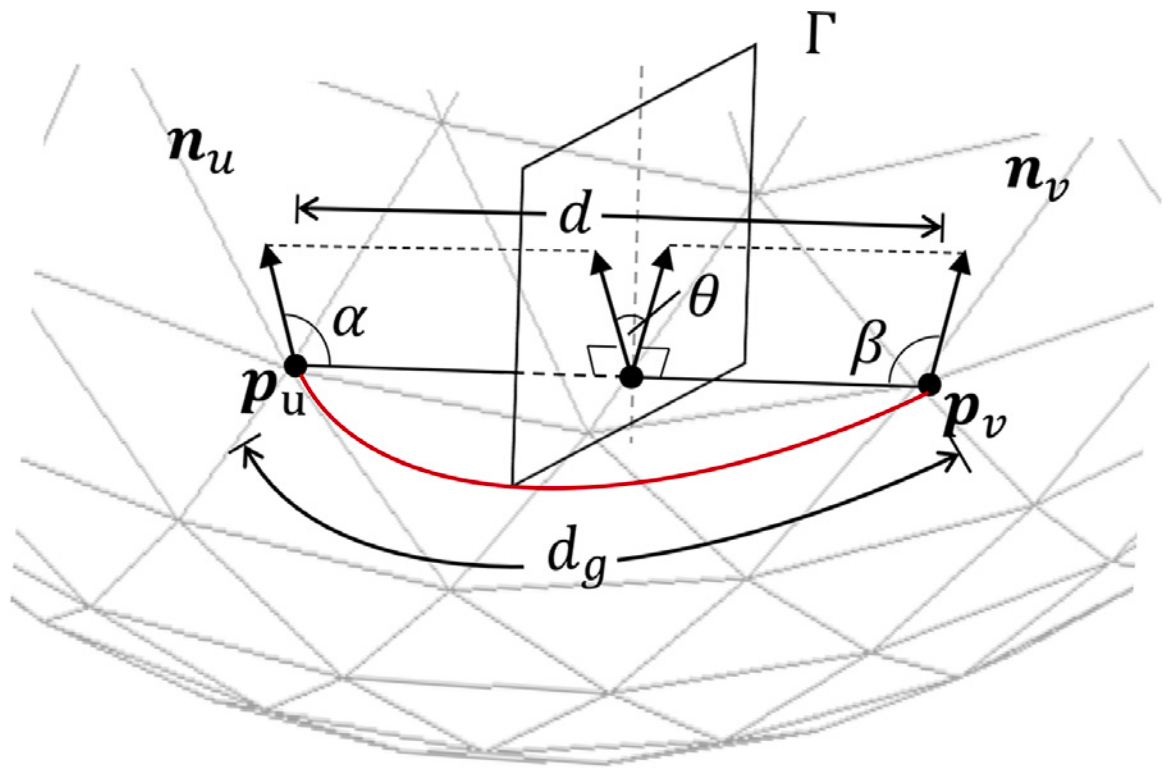
\includegraphics[scale=0.18]{images/espr.png}
    \caption{Parámetros de ESPR entre los puntos $p_u$ y $p_v$ \cite{5}}
    \label{fig:espr}
\end{figure}

\subsection{Descriptor de covarianza}
El descriptor de covarianza de un \textit{keypoint} $p$ está definido por la ecuación \ref{eq:20}, donde $p$ es comparado a sus vecinos en un radio $r$. En la ecuación, $\phi_p_i$ representa el vector característico del punto $p_i$, y $\mu$ el promedio de los vectores característicos  de los vecinos de $p$. El vector $\phi_p_i$ está descrito en \ref{eq:21}, donde los tres primeros parámetros representan las características locales de $p_i$, los siguientes tres representan las características globales y $H$ es la curvatura promedio en el punto \cite{6}.

\begin{equation} \label{eq:20}
    C_r (\phi(p, r)) = \frac{1}{N-1} \sum_{i=1}^{N} (\phi_p_i - \mu) (\phi_p_i - \mu)^T
\end{equation}
\begin{equation} \label{eq:21}
    \phi_p_i = \{ \cos{\alpha}, \cos{\beta}, \cos{\gamma}, \delta_1(p), \delta_2(p), \delta_3(p), H(p) \}
\end{equation}


\subsection{Descriptor \textit{2D link-chain} (LCD)}
El descriptor LCD de un borde $s_i$ está formado por los segmentos lineales de la curva de las superficies fracturadas. Para representar la secuencia de segmentos se utiliza la longitud $l_j$ y los ángulos internos $\theta_j$ entre segmentos adyacentes. El descriptor está representado en la ecuación \ref{eq:22} \cite{7}.
% y se ilustra visualmente en la imagen \ref{fig:lcd} \cite{7}.

\begin{equation} \label{eq:22}
    \mathbf{d_{s_i}} = (l_1, \mathbf{\theta_1}, l_2, \mathbf{\theta_2}, ...)
\end{equation}
\begin{comment}
\begin{figure}[!h]
    \centering
    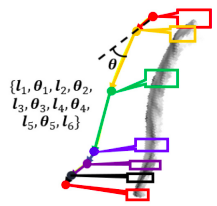
\includegraphics[scale=0.4]{images/lcd.png}
    \caption{Descriptor \textit{2D link-chain} \cite{7}}
    \label{fig:lcd}
\end{figure}
\end{comment}


\subsection{Descriptor \textit{3D spatial-distribution} (SDD)}
El descriptor SDD, descrito en la ecuación \ref{eq:25}, es calculado para cada área sobrepuesta entre las superficies $s_i$ y $s_j$.  Las características de linearidad $li$, planaridad $pl$, omnivarianza $om$ y anisotropía $an$ del descriptor son calculadas a partir de los eigenvalores $\lambda_1$, $\lambda_2$ y $\lambda_3$ de la superficie, como se muestra en las ecuaciones en \ref{eq:24} \cite{7}.

\begin{equation} \label{eq:23}
    \bar{\lambda} = \frac{\lambda_i}{\sum_{i=1}^{3} \lambda_i}
\end{equation}
\begin{equation} \label{eq:24}
    li = \frac{\bar{\lambda_1}-\bar{\lambda_2}}{\bar{\lambda_1}};
    \ \ pl = \frac{\bar{\lambda_2}-\bar{\lambda_3}}{\bar{\lambda_1}};
    \ \ om = \sqrt[3]{\bar{\lambda_1}*\bar{\lambda_2}*\bar{\lambda_3}};
    \ \ an = \frac{\bar{\lambda_1}-\bar{\lambda_3}}{\bar{\lambda_1}}
\end{equation}
\begin{equation} \label{eq:25}
    \mathbf{D_{m_{s_i}}} = (li_{m_{s_i}}, pl_{m_{s_i}}, om_{m_{s_i}}, an_{m_{s_i}})
\end{equation}


\section{Correspondencia}

La correspondencia de objetos 3D consiste en mapear los puntos de un modelo $X$ en una posición $M$ a una posición $N$ a través de una transformación $T$. La transformación se define formalmente en la ecuación \ref{eq:3}, donde $f$ y $g$ son los descriptores de $M$ y $N$ respectivamente \cite{17}.

\begin{equation} \label{eq:3}
    f:M \xrightarrow{} \mathbb{R}^n; \ \ \ \ \ T_F (f) = g:N \xrightarrow{} \mathbb{R}^n
\end{equation}

De manera similar, con una transformación diferente, el problema entre posiciones se convierte en el mapeo de una cara fracturada $X$ a una cara $Y$. Entonces, la correspondencia en el reensamblaje consiste en emparejar los fragmentos de un conjunto inicial de tal manera que se puedan unir y formar un nuevo fragmento, como se muestra en la figura \ref{fig:correspondencia} \cite{2}. 

\begin{figure}[!h]
    \centering
    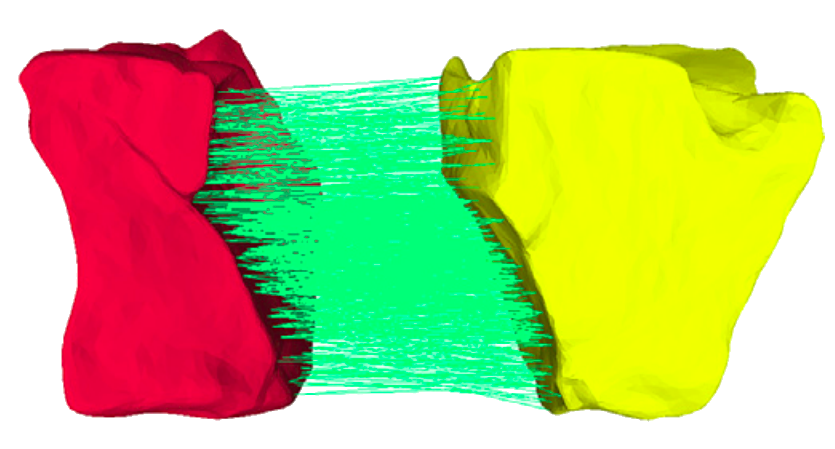
\includegraphics[scale=0.18]{images/correspondencia.png}
    \caption{Correspondencia entre fragmentos \cite{5}}
    \label{fig:correspondencia}
\end{figure}

\section{Alineación}
La alineación de objetos 3D consiste en encontrar la transformación rígida, compuesta por un vector de rotación $\hat{R}$ y un vector de traslación  $\hat{t}$, que minimiza la distancia entre las nubes de puntos $X$ y $Y$, dado el conjunto de correspondencias $M$. Formalmente, el problema está definido por la ecuación \ref{eq:4}, donde $g$ representa la transformación, y $d$ es el error entre $X$ y $Y$ transformado \cite{9}. 

\begin{equation} \label{eq:4}
    \argmin_{\hat{R}, \hat{t}}||d(X, g(Y))||^2_2 \ ; \ \ \ \ \ g(Y) = \hat{R}Y + \hat{t}
\end{equation}

En el problema de reensamblaje, la alineación también debe minimizar el \textit{overlapping} entre las nubes de puntos para hallar la mejor transformación. Además, la alineación puede tener dos etapas: una alineación global y una local \cite{2}. En la figura \ref{fig:alineacion}, se muestra la alineación entre dos caras de los fragmentos $X$ y $Y$, donde la transformación $T$ se aplica sobre el fragmento $X$.

\begin{figure}[!h]
    \centering
    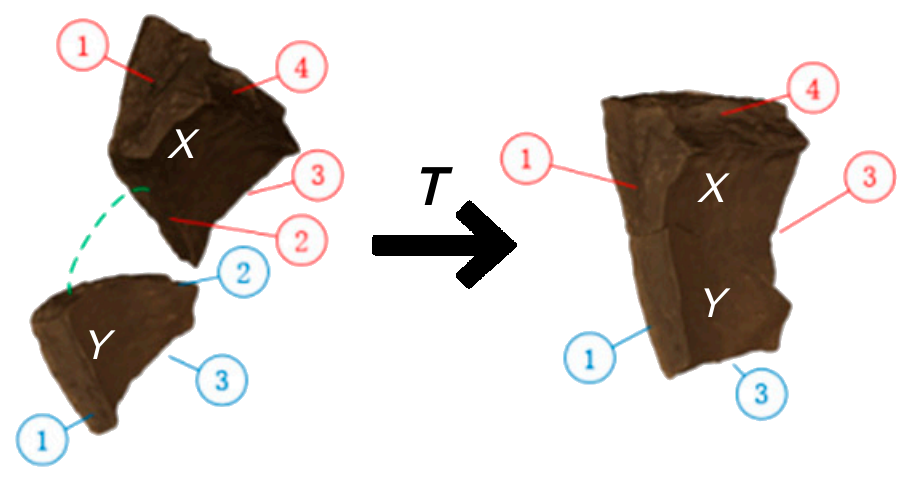
\includegraphics[scale=0.19]{images/alineacion.png}
    \caption{Alineación entre fragmentos \cite{6}}
    \label{fig:alineacion}
\end{figure}

\section{Redes neuronales}
\subsection{\textit{Pointnet}}
Es una arquitectura de red neuronal que recibe como entrada una nube de puntos para resolver tareas como clasificación de objetos o segmentación de partes, tal como se muestra en la figura \ref{fig:pointnet}. Primero, se inicia con una transformación de la entrada con una T-net para asegurar que sea invariante a transformaciones como rotación o traslación. Segundo, se extraen los vectores característicos de los puntos y se aplica una segunda transformación. Tercero, se emplea un \textit{multilayer perceptron} (MLP) y un \textit{max pooling} para asegurar que sea invariante al orden de los puntos de entrada. Con el vector de características globales obtenidas en el paso anterior, podemos agregar una MLP para clasificar objetos, o agregar las características locales para resolver la tarea de segmentación \cite{14}.

\begin{figure}[!h]
    \centering
     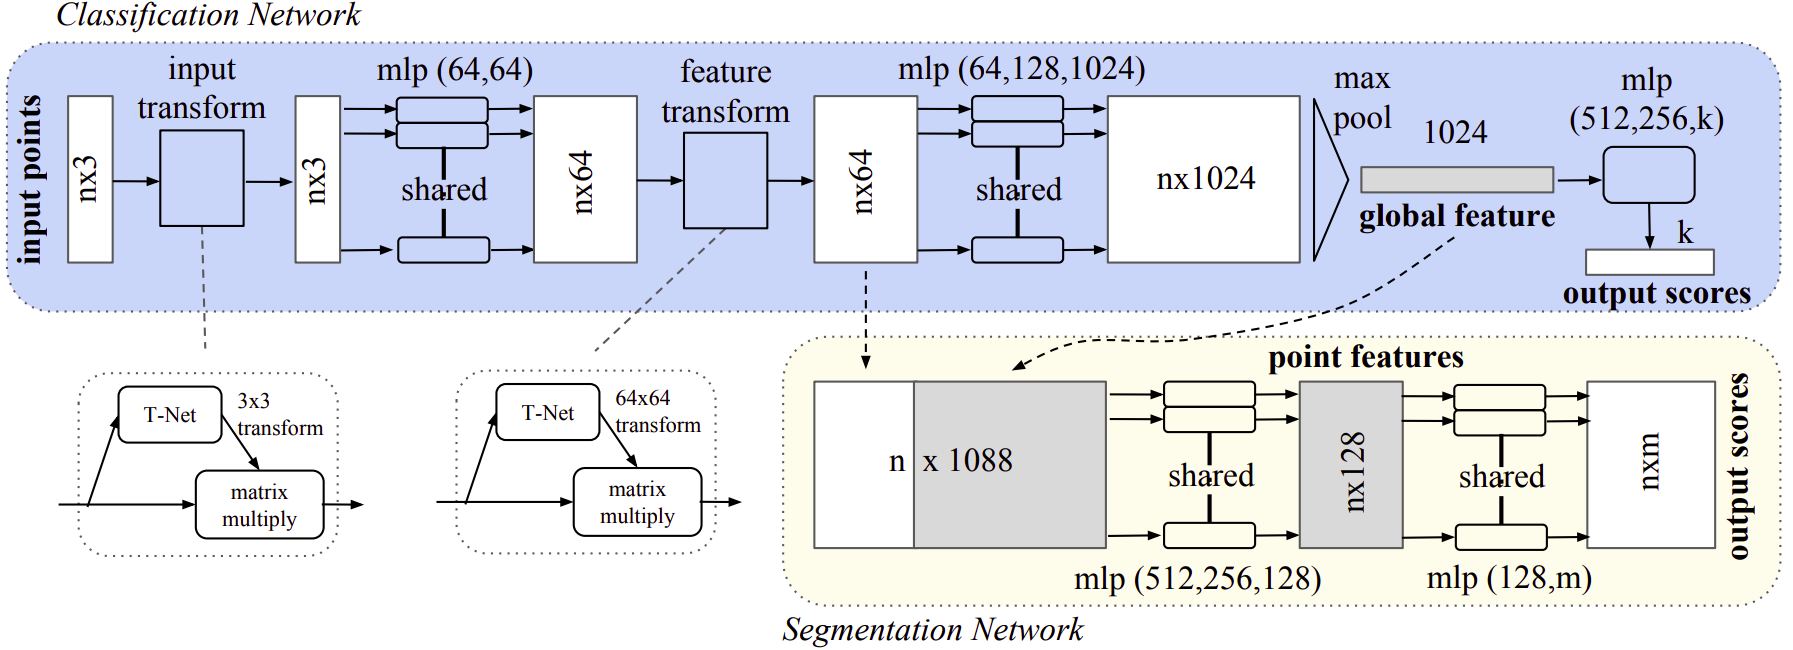
\includegraphics[scale=0.19]{images/pointnet.png}
    \caption{Arquitectura de la \textit{Pointnet} \cite{14}}
    \label{fig:pointnet}
\end{figure}

\subsection{Redes neuronales siamesas (SNN)}
Es una arquitectura compuesta por dos subredes neuronales idénticas que comparten el mismo conjunto de pesos. En la figura \ref{fig:snn} se muestra como cada red recibe una entrada diferente, de la cual extrae su respectivo vector característico. A continuación, los vectores característicos se comparan para determinar su similitud semántica a través de una función de pérdida de contraste. Además, SNN puede ser usado para resolver tareas como la verificación de imágenes, y detección de anomalías \cite{15}. 


\subsection{Funciones de pérdida}  \label{section:contrastive}
\subsubsection{Función de pérdida de contraste}
Dado dos vectores característicos $V_X$ y $V_Y$, y una etiqueta binaria $G$ que representa la similitud o diferencia entre ellos, se calcula la función de pérdida a través de la fórmula \ref{eq:41}. Para ello, se utiliza la distancia euclidiana y dos pérdidas parciales $L_s$ y $L_d$ como se muestra en \ref{eq:40} y \ref{eq:42}. Las pérdidas parciales se encargan de cubrir los casos de etiquetas similares y diferentes con un margen $m$ dentro del cual consideramos a dos vectores similares \cite{19}. 

\begin{equation} \label{eq:40}
    D_w = ||V_{X} - V_{Y}||_2
\end{equation}
\begin{equation} \label{eq:42}
    loss = G * L_s(D_w) + (1 - G) * L_d(D_w) 
\end{equation}
\begin{equation} \label{eq:41}
    loss = G * D_w^2 + (1 - G) * max(0, m - D_w)^2
\end{equation}

\begin{figure}[!h]
    \centering
     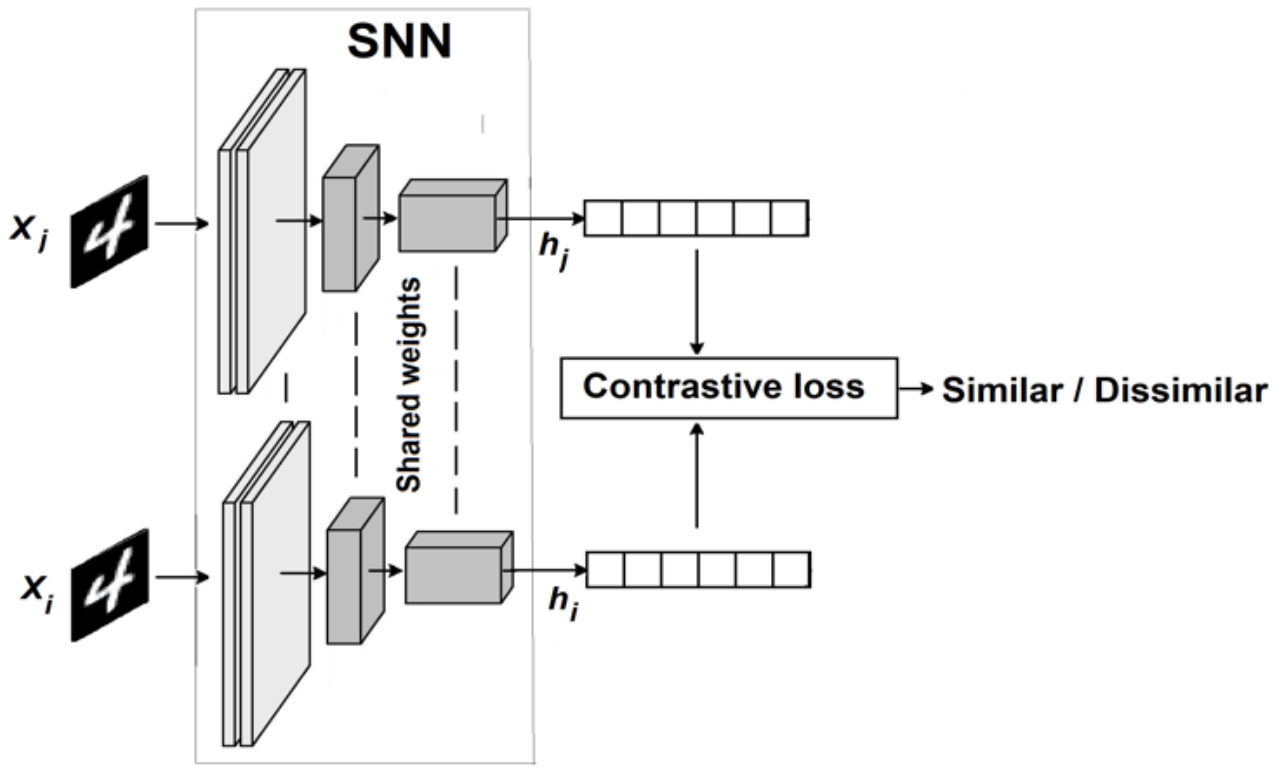
\includegraphics[scale=0.17]{images/snn.png}
    \caption{Arquitectura de la \textit{SNN} \cite{15}}
    \label{fig:snn}
\end{figure}


\hfill \break
\indent En este capítulo, se definieron conceptos importantes como correspondencia y alineación dentro del proceso de reensamblaje. Además, se revisaron los descriptores y redes neuronales involucradas en el proceso.
